%%%%%%%%%%%%%%%%%%%%%%%%%%%%%%%%%%%%%%%%%%%%%%%%%%%%%%%%%%%%%%%%%%%%%%
% Overleaf (WriteLaTeX) Example: Molecular Chemistry Presentation
%
% Source: http://www.overleaf.com
%
% In these slides we show how Overleaf can be used with standard 
% chemistry packages to easily create professional presentations.
% 
% Feel free to distribute this example, but please keep the referral
% to overleaf.com
% 
%%%%%%%%%%%%%%%%%%%%%%%%%%%%%%%%%%%%%%%%%%%%%%%%%%%%%%%%%%%%%%%%%%%%%%

\documentclass{beamer}

\mode<presentation>
{
  \usetheme{Madrid}       % or try default, Darmstadt, Warsaw, ...
  \usecolortheme{default} % or try albatross, beaver, crane, ...
  \usefonttheme{default}    % or try default, structurebold, ...
  \setbeamertemplate{navigation symbols}{}
  \setbeamertemplate{caption}[numbered]
} 

\usepackage[english]{babel}
\usepackage[utf8x]{inputenc}
\usepackage{chemfig}
\usepackage[version=3]{mhchem}

\usepackage{hyperref}
  \hypersetup{colorlinks=true}
  \hypersetup{urlcolor=blue}
  \hypersetup{linkcolor = .}
\usepackage{xcolor}
\usepackage{siunitx}
  \sisetup{separate-uncertainty = true}
\usepackage{physics}
\usepackage[font=small,labelfont=bf]{caption}
\usepackage{subcaption}
\usepackage[en-GB]{datetime2}
\usepackage{overpic}
\usepackage{feynmp}
\DeclareGraphicsRule{*}{mps}{*}{}

\usepackage{scalerel}
\newcommand{\mylbrace}[2]{\vspace{#2pt}\hspace{6pt}\scaleleftright[\dimexpr5pt+#1\dimexpr0.06pt]{\lbrace}{\rule[\dimexpr2pt-#1\dimexpr0.5pt]{-4pt}{#1pt}}{.}}
\newcommand{\myrbrace}[2]{\vspace{#2pt}\scaleleftright[\dimexpr5pt+#1\dimexpr0.06pt]{.}{\rule[\dimexpr2pt-#1\dimexpr0.5pt]{-4pt}{#1pt}}{\rbrace}\hspace{6pt}}

% Here's where the presentation starts, with the info for the title slide
\title[BESIII Oxford]{BESIII Oxford Group Meeting}
\author{Martin Tat}
\institute{Oxford LHCb}
\date{27th January 2022}

\titlegraphic{
\includegraphics[width = 4cm, height = 2.8cm]{lhcb.jpg}\hspace{1cm}~%
              
\includegraphics[width = 4cm, height = 2.8cm]{bes3.jpg}}

\begin{document}

\begin{frame}
  \titlepage
\end{frame}

% These three lines create an automatically generated table of contents.
%\begin{frame}{Outline}
%  \tableofcontents
%\end{frame}

\section{Loose IP cuts study}

\begin{frame}{Low kaon tag efficiency}
  \begin{itemize}
    \setlength\itemsep{1.5em}
    \item{Kaon efficiency very poor in 4-body modes}
    \begin{itemize}
      \item{$\pi\pi\pi\pi$: $49\%$}
      \item{$K\pi\pi\pi$: $37\%$}
      \item{$KK\pi\pi$: $18\%$}
    \end{itemize}
    \item{2-body modes do not show this trend:}
    \begin{itemize}
      \item{$\pi\pi$: $69\%$}
      \item{$K\pi$: $67\%$}
      \item{$KK$: $64\%$}
    \end{itemize}
  \end{itemize}
\end{frame}

\begin{frame}{Tracking efficiencies}
  \begin{figure}
    \centering
    \begin{subfigure}{0.49\textwidth}
      \centering
      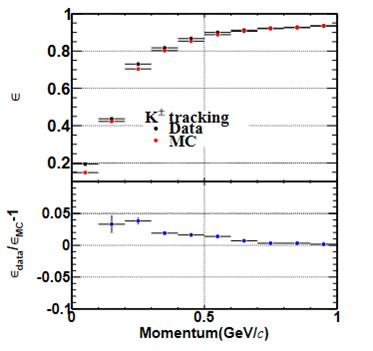
\includegraphics[width=\textwidth]{Plots/KaonEfficiency.jpg}
      \caption{$K^\pm$ tracking efficiency}
    \end{subfigure}%
    \begin{subfigure}{0.49\textwidth}
      \centering
      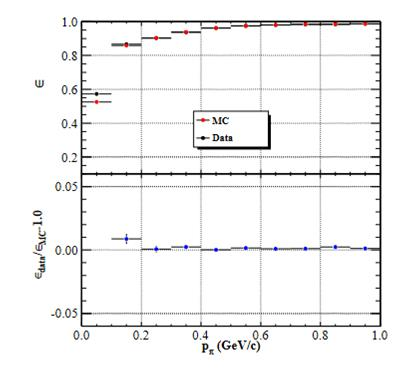
\includegraphics[width=\textwidth]{Plots/PionEfficiency.jpg}
      \caption{$\pi^\pm$ tracking efficiency}
    \end{subfigure}
  \end{figure}
  \begin{center}
    Maybe kaons get caught by magnetic field in MDC and decay?
  \end{center}
\end{frame}

\begin{frame}{Softer kaon momentum in $KK\pi\pi$}
  \begin{figure}
    \centering
    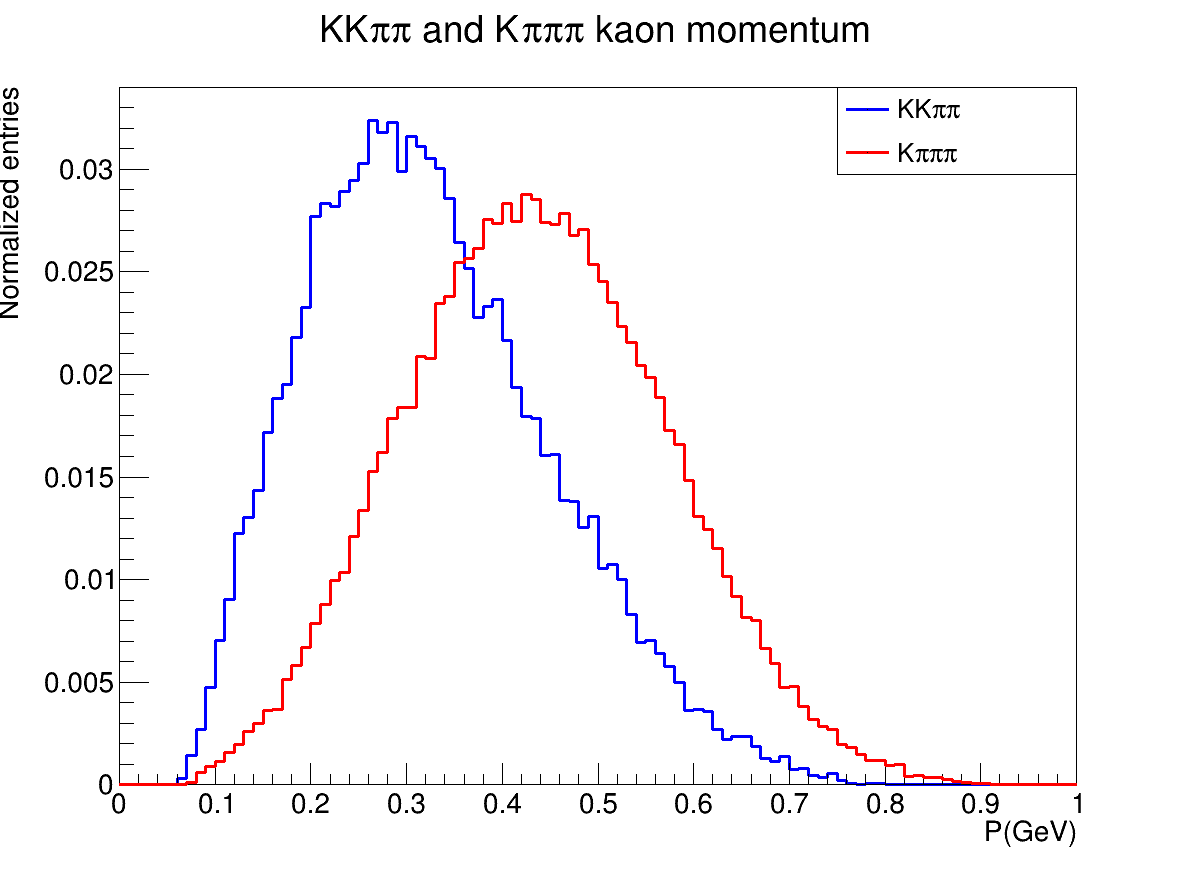
\includegraphics[width=0.9\textwidth]{Plots/KaonMomentum.png}
    \caption{Kaon momentum in $KK\pi\pi$ and $K\pi\pi\pi$}
  \end{figure}
\end{frame}

\begin{frame}{Study IP cuts}
  \begin{figure}
    \centering
    \begin{subfigure}{0.49\textwidth}
      \centering
      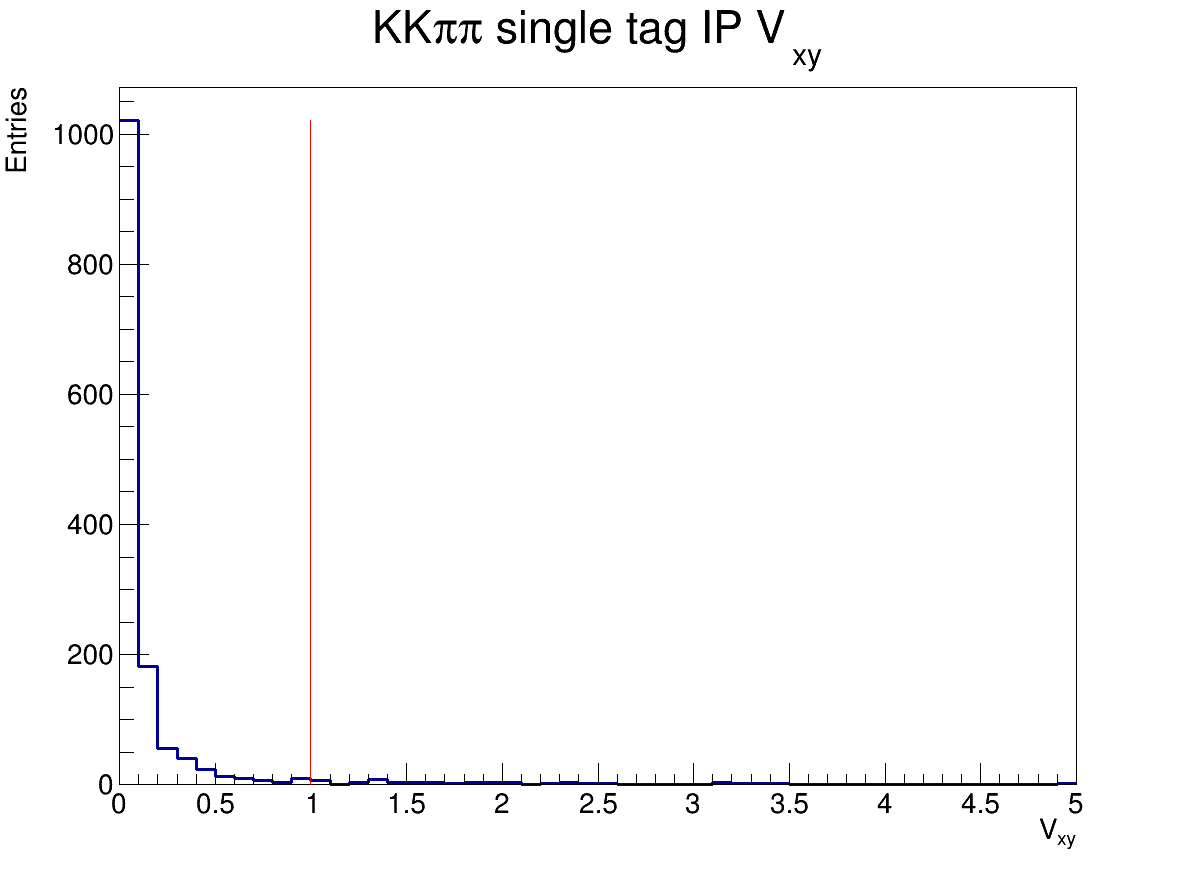
\includegraphics[width=\textwidth]{Plots/KaonIP_Vxy.png}
      \caption{Kaon $V_{xy}$}
    \end{subfigure}%
    \begin{subfigure}{0.49\textwidth}
      \centering
      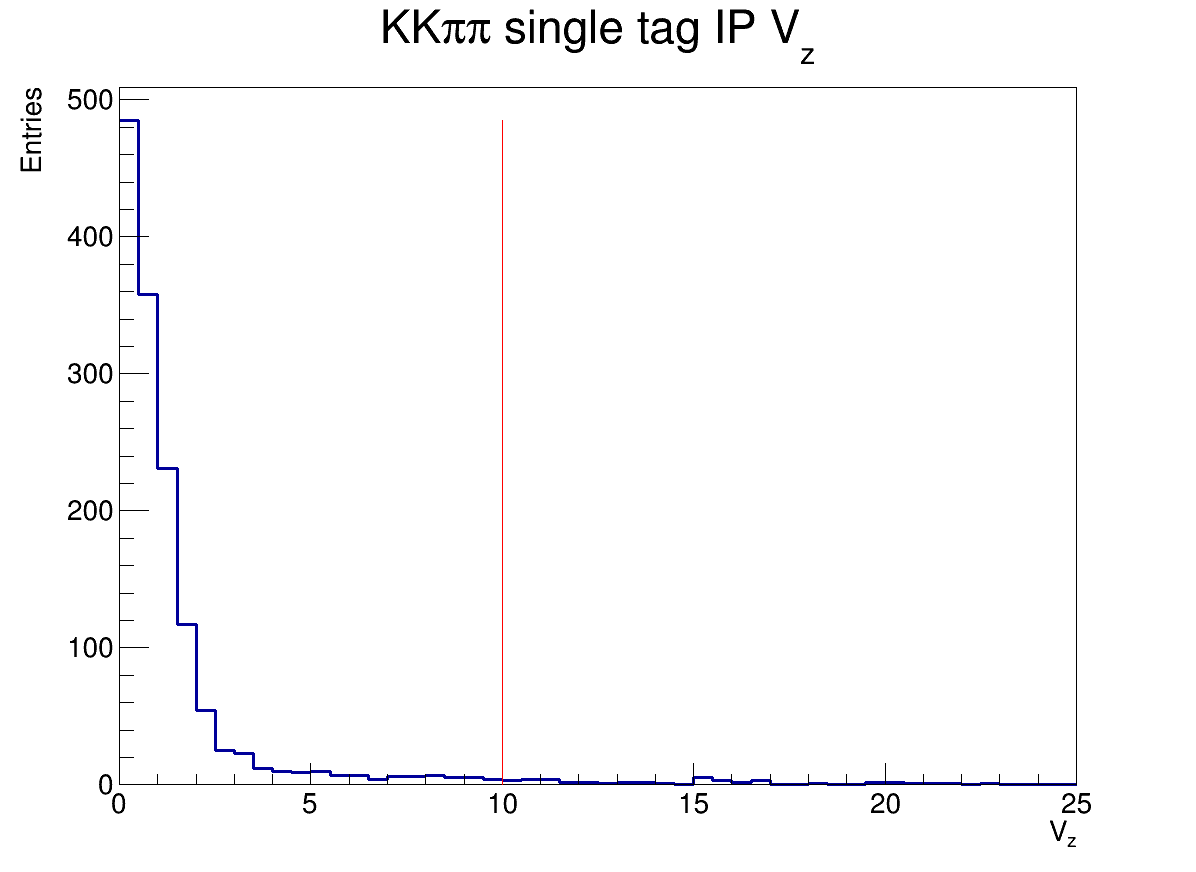
\includegraphics[width=\textwidth]{Plots/KaonIP_Vz.png}
      \caption{Kaon $V_z$}
    \end{subfigure}
  \end{figure}
  \begin{center}
    Removing IP cuts increases yields by $4.4\%$ \\
    Almost no change in tag efficiency...
  \end{center}
\end{frame}

\begin{frame}{Larger backgrounds without IP cuts}
  \begin{figure}
    \centering
    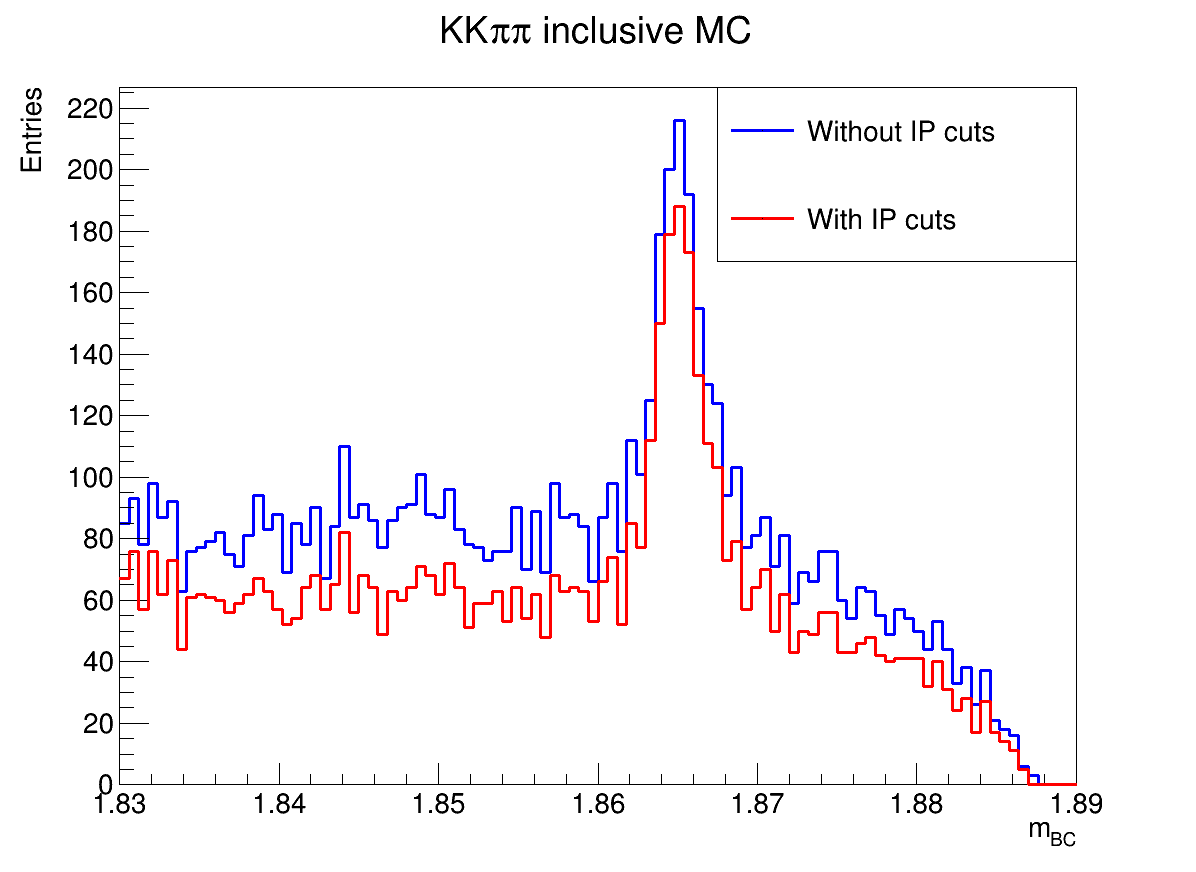
\includegraphics[width=0.9\textwidth]{Plots/InclusiveMC_IPcuts.png}
    \caption{$KK\pi\pi$ single tag in inclusive MC}
  \end{figure}
\end{frame}

\section{Next steps}
\begin{frame}{Conclusion}
  \begin{itemize}
    \setlength\itemsep{1.5em}
    \item{Minor gains from loosening IP cuts}
    \item{Instead: Partially reconstructed tag $KK\pi\pi$ where $K^\pm$ is missing}
    \item{Especially important for $K_S\pi\pi$ tags}
  \end{itemize}
\end{frame}

\end{document}
